\documentclass[12pt]{article}

\usepackage[figures]{uproject}
\usepackage[utf8]{inputenc}
\usepackage{epsfig}
\usepackage{amsmath}
\usepackage{listings}
\usepackage{color}

\definecolor{bluekeywords}{rgb}{0.13,0.13,1}
\definecolor{greencomments}{rgb}{0,0.5,0}
\definecolor{turqusnumbers}{rgb}{0.17,0.57,0.69}
\definecolor{redstrings}{rgb}{0.5,0,0}

\lstdefinelanguage{FSharp}
                {morekeywords={new, match, with, rec, open, module, namespace, type, of, member, and, for, in, do, begin, end, fun, function, try, mutable, if, then, else, maybe, return, let},
    keywordstyle=\color{bluekeywords},
    sensitive=false,
    morecomment=[l][\color{greencomments}]{///},
    morecomment=[l][\color{greencomments}]{//},
    morecomment=[s][\color{greencomments}]{{(*}{*)}},
    morestring=[b]",
    stringstyle=\color{redstrings}
    }
\lstset{
      language=FSharp,
      basicstyle=\ttfamily,
      breaklines=true,
      columns=fullflexible
    }

\title{Projektový seminář}
\subtitle{Latrunculi}
\author{Ondřej Grätz}
\group{Aplikovaná informatika, III. ročník}
\date{Červen 2016}

\docinfo{Ondrej Gratz}{Latrunculi}

\abstract{Implementace deskové hry Latrunculi s~použitím \emph{.NET Framework} pro~operační systém \emph{Windows}.}

\begin{document}
\maketitle

\newpage
\section{Zadání projektu}
Cílem projektu je vytvoření hry pro desktopový operační systém s~grafickým uživatelským rozhraním (GUI) dle standardů.

Požadavek na přenositelnost spustitelných souborů nebyl stanoven. Uživatelské rozhraní se~předpokládá objektově orientované s~použitím oken a~standardních prvků (hlavní nabídka, nástrojová lišta, tlačítka).

\section{Volba technologie}
\subsection{Výběr operačního systému}
Já jsem pro vývoj i~běh hry (aplikace) zvolil operační systém \emph{Windows}, jelikož je~mi~dobře známý a~také proto, že je to s~podílem 52~\% (viz~\cite{wiki2016}) mezi uživateli i programátory nejpoužívanější operační systém pro osobní počítače.

\subsection{Výběr vývojového prostředí}
Pro vývoj byl zvolen nástroj \emph{Visual Studio} od firmy \emph{Microsoft}, jazyky \emph{C\#} a~\emph{F\#} a~pro vývoj uživatelského rozhraní \emph{Windows Presentation Framework} (WPF).

Pro zvolený operační systém (\emph{Windows}) by~s~ohledem na~zadání bylo výhodné použít jeden z~následujících typů aplikací. 
	\begin{itemize}  
		\item Win32 (Visual C++ s použitím Windows API nebo MFC)
		\item .NET Framework + WinForms
		\item .NET Framework + WPF
		\item Windows Runtime (C++/CX) 
	\end{itemize}

\emph{Win32} a \emph{Windows Runtime} poskytují nejmenší úroveň abstrakce. Vývoj tohoto typu aplikací vyžaduje větší znalosti a~zkušenosti programátora. \emph{Windows Runtime} aplikace je navíc možné spustit pouze pod~operačním systémem \emph{Windows~8} (nebo novějším). Výhodou je ale standardní vzhled výsledných aplikací a~nejlepší výpočetní výkon.

Použití \emph{WinForms} by bylo výhodné, jelikož vývoj je jednoduchý (údálostmi řízený, objektově orientovaný). Výsledná aplikace má~vzhled v~souladu se~standardy operačního systému a~očekáváním uživatele. Nevýhodou je~strohý design, který se~příliš nepřizpůsobuje rozlišení obrazovky a~jehož vzhled se~může jevit zastaralý. Design je~navíc velmi svázán s~kódem, který má~na~starosti výpočty a~samotnou logiku aplikace.

Naproti tomu u~\emph{WPF} je již při vývoji myšleno na responzivní design. Prvky uživatelského rozhraní mají velmi bohaté a~pro programátora snadno použitelné vlastnosti, které umožňují přízpůsobit aplikaci různým velikostem obrazovky a~různým způsobům vstupu od uživatele (dotykové obrazovky, přizpůsobení pro zrakově nebo tělesně hendikepované uživatele). Návrh uživatelského rozhraní je~navíc velmi dobře oddělen od samotného kódu a~umožňuje s~použitím nástroje \emph{Microsoft Blend} výrazně zasáhnout do designu aplikace i~grafikovi (bez nutnosti znalosti programování a~bez zásahu do~modelu aplikace).

\section{Organizace kódu}
\subsection{Zvyklosti pro .NET aplikace}
Při vývoji pro \emph{.NET Framework} je nutno veškerý kód umisťovat do metod tříd. Třídy musejí být povinně organizovány do jmenných prostorů. Jmenné prostory je~vhodné stromově strukturovat dle~navržené architektury aplikace.

Pro \emph{.NET} aplikace (s výjimkou aplikací v jazyku F\#) je~typické rozdělení zdrojového kódu do~několika projektů, které jsou přidány do~skupiny projektů (Solution). Rozdělení se~provádí na~základě jmenných prostorů (\texttt{namespaces}) tak, aby třídy patřící do stejného prostoru byly ve~stejném projektu. 

Spustitelný (EXE) soubor obsahje jádro programu a~definice hlavních částí uživatelského rozhraní, ale komponenty uživatelského rozhraní i~třídy obsahující doménový nebo datový model, rozhodovací logiku a~třídy pro práci se soubory, databázemi či~síťovou komunikaci jsou umístěny v~tzv.~knihovnách tříd (DLL soubory). Toto dělení poté představuje výhodu při požadavku na~změnu typu výsledné aplikace. Lze například textové rozhraní aplikace nahradit GUI. Nebo nahradit samostatně spustitelnou konzolovou aplikaci službou systému Windows. Společné součásti tak mohou být opětovně využívány (sdíleny).

DLL~i~EXE soubory po sestavení obsahují překladačem vytvořený \emph{bytecode}, který je~poté při spuštění aplikace částečně kompilován do strojového kódu (just-in-time kompilace) a~částečně také interpretován běhovým prostředím \emph{.NET}.

\subsection{Prevence cyklických závislostí}
Abstraktní rozdělení kódu na vrstvy pomáhá při vývoji předcházet cyklickým (rekurzivním) závislostem mezi třídami (respektive mezi jednotlivými knihovnami tříd). Nevhodné závislosti mezi třídami by~totiž mohly při dokončování aplikace způsobit komplikace, které by~v~krajním případě bránily sestavení aplikace a~vyžadovaly by~refaktorování celého kódu.

Jako prevence se~proto činnosti jednotlivých součástí seskupují tak, aby vyšší vrstvy byly závislé na nižších vrstvách. Nevhodné je naopak odkazovat se~z~nižších vrstev na~vyšší, ačkoliv i~tato možnost může být potřebná. V~případě potřeby se~ale namísto reference používají události tak, že nižší vrstva generuje událost a~vyšší vrstva událost zachytává. Bližší informace viz~\cite{wlaschin1}.

\subsection{Soubory projektu}
Třídy projektu jsou organizovány v~podprostorech jmenného prostoru \texttt{Latrunculi}. 

Rozvrstvení aplikace je~zobrazeno na~obr.\ref{Layers} Výsledné soubory sestavení jednotlivých projektů (assemblies) a~jejich závislosti jsou zobrazeny na~obr.\ref{Assemblies} Rozdělení do~více projektů bylo provedeno s~ohledem na~výše uvedené zásady.

Úlohy jednotlivých částí systému budou popsány v~další kapitole.

\begin{figure}[ht]
  \centering
  \begin{minipage}[b]{0.4\textwidth}
		\center{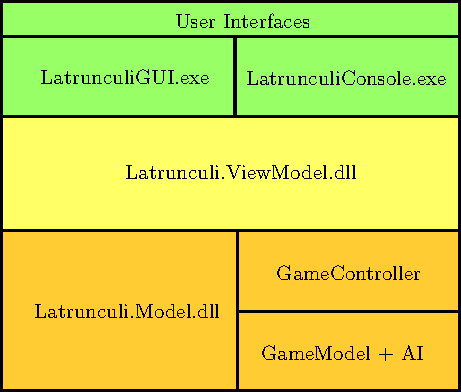
\includegraphics[height=60mm]{Layers.pdf}}
		\caption{Vrstvy aplikace}
		\label{Layers}
  \end{minipage}
  \hfill
  \begin{minipage}[b]{0.4\textwidth}
		\epsfysize=70mm
		\center{\epsfbox{Assemblies.eps}}
		\caption{Závislosti souborů}
		\label{Assemblies}
  \end{minipage}
\end{figure}

\section{Vrstvy aplikace}
Rozvrstvení aplikace vychází z architektury \texttt{MVC} (\emph{Model-View-Controller}, viz \cite{mvc}). Pro vývoj \emph{WPF} aplikace jsem jej ale musel mírně modifikovat. Úlohu pohledu (\texttt{View}) zastává~konkrétní okno aplikace (instance třídy \texttt{System.Windows.Window}) nedělitelně spolu s~odpovídajícím pohledovým modelem (\texttt{ViewModel}), jehož instanci okno vytvoří ve~svém konstruktoru. Výsledkem je~\texttt{MWVmC}, tj.~\emph{Model-Window-ViewModel-Controller}.

\subsection{Uživatelské rozhraní \texttt{(Latrunculi*.exe)}}
Nejvyšší vrstvou v našem diagramu z~obr.\ref{Layers} je \emph{User Interfaces}, tj. uživatelská rozhraní. Vrstva je~horizontálně rozdělena, neboť naše aplikace má dva typy samostatně spustitelných uživatelských rozhraní. Konzolové rozhraní (\texttt{Latrunculi.ConsoleUI}) a~grafické rozhraní (\texttt{Latrunculi.GUI}).

Uživatelské rozhraní zobrazuje stav hry uživateli a~poskytuje prvky pro ovládání hry. Neobsahuje ale samotnou logiku ani řízení hry. Požadavky od~uživatele jsou předávány nižší vrstvě - \texttt{GameController}.

Konstruktoru hlavního okna aplikace je nutno předat vytvořené instance tříd z~nižších vrstev - \texttt{MainWindowViewModel}, \texttt{GameController}. Za~vytvoření jejich instancí zodpovídá třída, která okno vytváří. V~našem případě třída \texttt{App} (vstupní bod aplikace).

\subsection{Pohledový model \texttt{(Latrunculi.ViewModel.dll)}}
Použití pohledových modelů je typické pro WPF aplikace. Úlohou pohledového modelu je poskytnout uživatelskému rozhraní třídy, které obsahují vlastnosti (\emph{Properties}), jež mohou být přímo napojeny na~jednotlivé grafické komponenty uživatelského rozhraní. Takové třídy musejí implementovat rozhraní \texttt{INotifyPropertyChanged}, tj. implementovat událost \texttt{PropertyChanged}. Tato událost je~zachytávána uživatelským rozhraním. 

Při zachycení události dojde automaticky  k~aktualizaci grafických komponent, které jsou navázány (\texttt{Binding})  na vlastnost třídy, jejíž hodnota byla změněna. Dodejme navíc, že~je~podporováno i~zachytávání změn v~generických kolekcích typu \texttt{ObservableCollection<T>}, což se~využívá pro aktualizaci komponent GUI typu List, ComboBox či tabulkového zobrazení.

Podobný princip aktualizace komponent (využití Bindingu) existuje i~v~aplikacích \emph{WinForms} a~také i~v~jiných vývojových prostředích a~jazycích (Delphi, Java). Smyslem je odstranit nutnost psát kód, který nesouvisí přímo s~výpočetní logikou aplikace či~jejím doménovým modelem.

Příkladem takového kódu je např. v události \texttt{Form.OnShow} kód \texttt{textBox1.Text = "Test"; }, kterým se zaktualizuje konkrétní komponenta. Pokud komponentu \texttt{textBox1} přejmenujeme nebo odstraníme, aplikace přestane fungovat a~daný řádek musíme upravit. Při použití pohledového modelu ve~\emph{WPF} aplikaci nemusí mít komponenta vůbec stanovený název a~navíc může být více komponent (i~různých typů) navázáno na stejnou vlastnost v~třídě pohledového modelu. Jakákoliv změna v~návrhu uživatelského rozhraní nerozbije funkčnost pohledového modelu.

V pohledovém modelu se~zpravidla implementují třídy, které odpovídají třídám z~nižší vrstvy aplikace (z~doménového či datového modelu). Avšak implementují se~pouze ty~třídy, u kterých se~předpokládá nutnost grafické reprezentace. Tj. zobrazení uživateli ve formě odpovídajícího grafického prvku. Někdy může být výhodné sloučit vlastnosti z~různých tříd datového modelu do~jedné třídy pohledového modelu.

Pohledový model si~načítá a~transformuje data z~doménového modelu. Konstruktoru pohledového modelu proto musí být předána platná instance třídy \texttt{GameModel}.

\subsection{Kontrolér a doménový model \texttt{(Latrunculi.Model.dll)}}
Tyto součásti jsou implementovány v~jazyku F\#, který jakožto ryze funkcionální jazyk poskytuje možnosti interaktivního prototypově či doménově řízeného vývoje. Také obsahuje některé prostředky (např. datové typy a~struktury), které usnadňují vývoj aplikací, a~přitom v~jazyku C\# nemají odpovídající náhradu. Skriptovací vlastnosti jazyka F\# navíc využijeme pro testování jednotlivých součástí aplikace.

Kontrolér má na starosti~řízení hry. Jeho metody jsou volány z~uživatelského rozhraní. Kontrolér na~základě jejich volání provede příslušnou akci a~předá požadavek doménovému modelu. Toto zpravidla také povede ke~změně stavu modelu a~tudíž k~nutnosti aktualizovat pohledový model a~uživatelské rozhraní.

Doménový model reprezentuje samotnou hru Latrunculi. Jeho úkolem je modelovat reálnou podobu hry, včetně jejích entit (deska, figurka, hráč, pravidla) a~jejich atributů a~metod. Doménový model musí zajistit, aby se~hra neocitla ve~stavu který odporuje pravidlům nebo je~v~rozporu s~očekáváným chováním deskové hry. Více obecně o~doménově řízeném vývoji viz \cite{wlaschin2}.

Součástí této vrstvy je i~implementace mozku počítačového hráče (\texttt{AI}).

\section{Návrh aplikace}
\subsection{Případy užití}
Případy užití vycházejí ze zadání a jsou zobrazeny v příloze na obr.\ref{PrimaryUseCases} Někteří aktéři poslouží jako základ pro objekty modelu. Jednotlivé případy užití potom poslouží při implementaci metod daných objektů.

\begin{figure}[ht]
	\epsfysize=200mm
	\center{\epsfbox{PrimaryUseCases.eps}}
	\caption{Případy užití}
	\label{PrimaryUseCases}
\end{figure}

\subsection{Diagram tříd}
Hlavní třídy používané pro uživatelské rozhraní a~jejich atributy a~relace jsou uvedeny na~obr.\ref{UIClassDiagram}. Třídy doménového modelu nejsou uvedeny v~diagramu tříd, protože kvůli konstrukci jazyka F\#, vypovídající hodnotě kódu v~F\# a~prototypově řízeném vývoji nemá tvoření diagramu tříd při návrhu téměř žádnou přidanou hodnotu.

Třídy pohledového modelu nebudou v~textu probírány, protože jsou z~hlediska implementace nezajímavé (je~to~pouze ,,mechanický" kód  zapouzdřující data z~doménového modelu.

\begin{figure}[ht]
	\epsfysize=200mm
	\center{\epsfbox{UIClassDiagram.eps}}
	\caption{Diagram tříd}
	\label{UIClassDiagram}
\end{figure}

\subsection{Unit Testy}
Pro testování je použit framework \emph{NUnit 3.2.1}. Soubory s~testy doménového modelu jsou umístěny v~sestavení \texttt{Latrunculi.Model.Test.dll}.

\section{Implementace}
Po~vytvoření projektů \emph{Visual Studia} a nastavení jejich vzájemných referencí jsem započal implementaci. A~to~od~nejnižší vrstvy, tj. doménového modelu. Pro implementaci ve~vývojovém prostředí bylo využito okno \emph{F\# Interactive}, které zpřístupňuje \texttt{REPL} cyklus jazyka F\#. Bez nutnosti kompilace, spuštění či ladění nebo vytvoření zdrojového souboru umožňuje přímo zadat požadovanou definici objektu a~ihned objekt otestovat (vytvořit instanci), případně doupravit.

V~následujícím popisu jednotlivých součástí uvádím ve~zdrojovém kódu především názvy významných atributů a~významné funkce a~jejich parametry. Tedy ne~celý zdrojový kód (s~výjimkou entity \texttt{Piece}, jejíž kód je uveden pro ilustraci).

\subsection{Modul \texttt{Common}}
Obsahuje definice společné pro celý model a kontrolér. Např. podporu návratových hodnot funkcí a~podporu výpočtových funkcí (monáda \texttt{Maybe}).
\begin{lstlisting}[language=FSharp]
[<AutoOpen>]
module Common

    type Result<'TSuccess,'TError> = 
        | Success of 'TSuccess 
        | Error of 'TError

    let getObjExn c =
        match c with
        | Success c -> c
        | _ -> failwith "Unable to extract object instance from function result, because called function has failed."

    type MaybeBuilder() =
        member this.Bind(x, f) = 
            match x with
            | Success s -> f s
            | Error e -> Error e

        member this.Return(x) = 
            x
\end{lstlisting}

\subsection{Entita \texttt{Piece}}
Tato entita je implementována jako strukturovaný typ \texttt{Record} jazyka F\#. Reprezentuje herní kámen, který bude umísťován na~hrací desku. Ve~hře Latrunculi je~pouze jeden typ kamenů, a~proto jediným atributem bude barva (bílá nebo černá).
Zdrojový kód:
\begin{lstlisting}[language=FSharp]
namespace Latrunculi.Model

module Piece =
    
    type Colors = 
        | White = 0
        | Black = 1

    [<StructuralEquality;NoComparison>]
    type T = {
        Color: Colors }
    
    let create x =
        { Color = x }
\end{lstlisting}
Pro představu, jak velkou abstrakci umožňuje jazyk F\# proti jazykům C\# či .NET Basic uvádím i~kód v~jazyku C\#, který implementuje stejnou funkcionalitu (vyžadovali jsme přímo porovnatelný, nemutovatelný strukturovaný objekt).

\begin{lstlisting}[language=C,basicstyle=\tiny]
using System;
using System.Collections;

namespace Latrunculi.Model
{
	[Serializable]
	public class Piece : IEquatable<Piece>, IStructuralEquatable
	{
		public Piece(PieceColors color)
		{
			Color = color;
		}
                    
		internal PieceColors Color;
		public PieceColors Color
		{
			get
			{
				return this.Color;
			}
		}
                   
		public override int GetHashCode(IEqualityComparer comp)
		{
			if (this != null)
			{
				int num = 0;
				return (int)(-1640531527 + (this.Color + ((num << 6) + (num >> 2))));
			}
			return 0;
		}
			
		public override int GetHashCode()
		{
			return this.GetHashCode(LanguagePrimitives.GenericEqualityComparer);
		}
		
		public override bool Equals(object obj, IEqualityComparer comp)
		{
			if (this == null)
			{
				return obj == null;
			}
			Piece t = obj as Piece;
			if (t != null)
			{
				Piece t2 = t;
				return this.Color == t2.Color;
			}
			return false;
		}
		
		public override bool Equals(Piece obj)
		{
			if (this != null)
			{
				return obj != null && this.Color == obj.Color;
			}
			return obj == null;
		}
		
		public override bool Equals(object obj)
		{
			Piece t = obj as Piece;
			return t != null && this.Equals(t);
		}
	}
}
\end{lstlisting}

Funkčně ekvivalentní kód v~jazyku C\# je výrazně delší.

\subsection{Entita \texttt{Square}}
Reprezentuje políčko na hrací desce. Je implementováno jako typ \texttt{discriminated union}. Políčko obsahuje buďto kámen nebo je prázdné.
\begin{lstlisting}[language=FSharp]
module Square =

    type T =
        | Piece of Piece.T
        | Nothing

    let isEmpty x =
        match x with
        | Nothing -> true
        | _ -> false

    let createWithPiece piece =
        Piece piece

    let createEmpty =
        Nothing
\end{lstlisting}

\subsection{Entita \texttt{Coord}}
Reprezentuje souřadnice. Obsahuje logiku pro kontrolu rozsahu souřadnic. Souřadnice je možné vytvořit z~řetězce (např. \texttt{"A1"}) nebo předání zvlášť písmene označující sloupec a~čísla řádku.
\begin{lstlisting}[language=FSharp]
module Coord =
    type Error =
        | InvalidColumnNumber
        | InvalidRowNumber
        | UnableToParseCoordFromString

    type ColumnNumber = ColumnNumber of char
    type RowNumber = RowNumber of int

    let ColumnNumbers = seq ['A'..'H']
    let RowNumbers = Seq.init 7 (fun i -> 7 - i) // [7..1]

    let ColIndex =
        Seq.fold (fun (i, xs) x -> 
                    (i + 1, (ColumnNumber x, i)::xs)) 
            (0, []) ColumnNumbers 
        |> snd |> List.rev |> Map.ofList
    let RowIndex =
        Seq.fold (fun (i, xs) x -> 
                    (i + 1, (RowNumber x, i)::xs)) 
            (0, []) RowNumbers 
        |> snd |> List.rev |> Map.ofList

    type T = {
        Column: ColumnNumber;
        Row: RowNumber }
        
    let tryCreate x y =
    let tryCreateFromString (s: string) =
\end{lstlisting}

\subsection{Entita \texttt{RemovedPiece}}
Zajatý kámen. Musíme si zaznamenat druh i~souřadnice kamene, který bude odebrán (resp. přidán) při provedení tahu (resp. inverzního tahu).
\begin{lstlisting}[language=FSharp]
module RemovedPiece =

    type T = {
        Coord: Coord.T;
        Piece: Piece.T }
    
    let create x y =
        { Coord = x; Piece = y }
\end{lstlisting}

\subsection{Entita \texttt{Move}}
Struktura \texttt{Record}, která reprezentuje tah a~obsahuje počáteční a~koncové souřadnice a~také nové stavy obou políček. Obsahuje také seznam zajatých kamenů a jejich souřadnic (kameny, které budou odstraněny z~hrací desky). Při~vytváření instance se~kontroluje, zda počáteční a~koncová souřadnice není shodná.
\begin{lstlisting}[language=FSharp]
module Move =
    type Error =
        | InvalidSourceCoordSpecified
        | InvalidTargetCoordSpecified
        | SourceAndTargetMayNotBeSame

    type T = {
        Source: Coord.T;
        Target: Coord.T;
        NewSourceSquare: Square.T;
        NewTargetSquare: Square.T;
        RemovedPieces: RemovedPiece.T list }

    let tryCreateWithRemovedPiecesList x y nx ny xys = ...

    let tryCreate x y nx ny =
        tryCreateWithRemovedPiecesList x y nx ny []
\end{lstlisting}

\subsection{Třída \texttt{Board}}
Hrací deska (Board) provádí tahy (bez ověřování pravidel), uchovává rozmístění kamenů a~provedné tahy ukládá do~historie.

Rozmístění kamenů je dvojrozměrné pole objektů \texttt{Square}.

\subsection{Třída \texttt{Latrunculi.Model.GameModel}}

\subsection{Třída \texttt{Latrunculi.Controller.GameController}}


\section{Systémové požadavky}
Pro vývoj i~běh aplikace jsou na počítač kladeny tyto nároky:
	\begin{itemize}  
		\item osobní počítač, notebook nebo tablet
		\item 32bitový (x86) nebo 64bitový (x64) procesor s frekvencí 1 GHz nebo vyšší
		\item operační systém Microsoft Windows 7 (64 bitový nebo 32 bitový)
		\item 1 GB paměti RAM (32bitová verze) nebo 2 GB paměti RAM (64bitová verze)
		\item 16 GB volného místa na disku (32bitová verze) nebo 20 GB (64bitová verze)
		\item Grafická karta s podporou DirectX 9 s ovladačem WDDM 1.0 nebo novějším
		\item Microsoft .NET Framework verze 4.5.2 (nebo novější)
	\end{itemize}

\section{Vytvoření aplikace}
\subsection{Instalace vývojového prostředí}
Pro sestavení aplikace nainstalujeme nejprve vývojové prostředí \emph{Microsoft Visual Studio}.

Pro vývoj byla použita edice \emph{Community 2015}, která je zdarma ke~stažení na stránce \url{https://www.visualstudio.com/cs-cz/downloads/download-visual-studio-vs.aspx}. 

Při instalaci zvolíme jazyk C\#. Po nainstalování zvolíme v menu File $\rightarrow$ New $\rightarrow$ Project... V zobrazeném dialogovém okně zvolíme ve~stromu vlevo položku Installed $\rightarrow$ Templates $\rightarrow$ Other Languages $\rightarrow$ Visual F\# a~poté v seznamu nabídnutých položek zvolíme Install F\# Tools a~provedeme instalaci nástrojů pro vývoj v~jazyku F\# (pokud máme již správně nainstalovánu podporu jazyku F\#, budou v~seznamu položky Console Application, Library a další).

Lze použít i~jiné edice, případně starší verze \emph{Visual Studia}. Jediným požadavkem je, aby daná verze uměla cílit na~\emph{.NET Framework verze 4.5.2} a~aby podporovala jazyk F\# verze 4.0.
\subsection{Sestavení aplikace}
Jestliže nemáme soubory se zdrojovým kódem, tak v nabídce Team zvolíme Manage Connections. V~okně Team Explorer - Connect v části Local Git Repositories zvolíme příkaz Clone a~jako Repository URL zadáme \url{https://github.com/ondrejgr/FLatrunculi.git}. Případně změníme název složky, do které chceme zdrojové soubory stáhnout.

Příkazem Build Solution v menu Build provedeme sestavení aplikace.

Pokud budeme chtít spouštět i testy, nainstalujeme \emph{NUnit} z \url{http://www.nunit.org/index.php?p=download}.

\section{Spuštění aplikace}
Aplikace se spouští spustitelným souborem \texttt{LatrunculiGUI.exe}. Ve~složce s~aplikací musejí být uloženy také následující soubory knihoven tříd:
	\begin{itemize}  
		\item \texttt{FSharp.Core.dll}
		\item \texttt{Latrunculi.Model.dll}
		\item \texttt{Latrunculi.ViewModel.dll}
	\end{itemize}

\newpage
\begin{thebibliography}{10}
	
\bibitem{outr2008} Mgr. Jan Outrata, Ph.D.: \emph{Projekt - implementace},
 \url{http://outrata.inf.upol.cz/courses/ps/navrh.pdf},
			listopad~2008.

	
\bibitem{outr2010} Mgr. Jan Outrata, Ph.D.: \emph{Projekt - analýza a návrh},
 \url{http://outrata.inf.upol.cz/courses/ps/implementace.txt},
			listopad~2010.

\bibitem{kuhr2011} Mgr. Tomáš Kühr, Ph.D.: \emph{Algoritmy realizující počítačového hráče},
 \url{http://www.inf.upol.cz/downloads/studium/PS/algoritmy.pdf},
			říjen~2011.

\bibitem{wiki2016}Wikipedia: \emph{Usage share of operating systems},
 \url{https://en.wikipedia.org/wiki/Usage_share_of_operating_systems#Desktop_and_laptop_computers},
			květen~2016.

\bibitem{mvc}Wikipedia: \emph{Model-view-controller},
 \url{https://en.wikipedia.org/wiki/https://en.wikipedia.org/wiki/Model-view-controller},
			květen~2016.

%%\bibitem{wlaschin}Scott Wlaschin: \emph{F\# For Profit And Fun},
 %%\url{https://fsharpforfunandprofit.com/},
%%			květen~2016.

\bibitem{wlaschin1}Scott Wlaschin: \emph{Dependency Cycles},
 \url{https://fsharpforfunandprofit.com/series/dependency-cycles.html},
			květen~2016.

\bibitem{wlaschin2}Scott Wlaschin: \emph{Domain Driven Design},
 \url{https://fsharpforfunandprofit.com/ddd/},
			květen~2016.

\end{thebibliography} 

\end{document}
